\chapter{[Microsoft] Web-Scale Generic Object Detection at Microsoft Bing}

\textbf{Reference:}~\url{https://arxiv.org/abs/2107.01814}

\textbf{Keywords:} visual search, objects detection, crowdsourcing

\section*{Какую задачу решают авторы?}

\textit{Visual Search (VS)} относительно новое направление в информационном поиске, в сравнении, например, с классическим текстовым поиском.
VS системы позволяют пользователю формулировать свой запрос в виде изображения.

Запрос пользователя может состоять как просто в поиске похожих изображений, так и в том, чтобы найти информацию касательно объектов, рассположенных на изображении.
Например, см. Рисунок~\ref{fig:bing_visual_search}, пользователь может загрузить изображение человека в куртке, и VS система поможет пользователю найти данную курту в интернет магазинах.

\begin{figure}[ht]
  \centering
  \includegraphics[width=0.8\linewidth]{images/bing_visual_search.png}
  \caption{\footnotesize{Examples of user interfaces with interactive hotspots}}
  \label{fig:bing_visual_search}
\end{figure}

С точки зрения ML, VS система в первую очередь решает задачу \textit{Objects Detection}~\cite{lin2017focal}. \\

Разработка VS систем~\cite{hu2018web,zhang2018visual} сопряжена с большим количеством челенджей, в частности:
\begin{itemize}
    \item \textbf{Data collection and processing for a large vocabulary} --- При разработке VS системы, способной распозновать большое кличество категорий объектов ($\sim 1000$), большая проблема состоит в сборе данных для обучения.
    
        Открытые датасеты с размеченными объектами имеют сильно разное распределение объектов в них, и их объединение не тривиально. 
        Ручная подготовка данных экспертами так же довольно затруднительна из-за большого количества возможных категорий объектов.
    \item \textbf{Agility of model development} --- На практике нередко возникает необходимость в том чтобы научится расспозновать новую категорию объектов. 
        При этом, с точки зрения бизнеса, необходимо чтобы не ухудшилось качество распознования уже имеющихся категорий.
    
        Переобучение массивной модели с нуля может представлять определенные трудности.
\end{itemize}

Авторы предлагают элегентное решение на основе \textit{crowdsourcing'a} для эффективной разметки данных для обучения модели, и архитектуру на основе  отдельных детекторов, для распознования объектов разных категорий, для того чтобы обновление моделей в продакшн окружении было более простым.

\section*{Как решают?}

Рассмотрим сначала подробнее то как авторы предлагают собирать данные для обучения, а затем архитуектуру детекторов объектов.

\subsection*{Data Collection}

Для получения разметки объектов на изображениях, можно попросить асессоров на crowd платформе просто выделить все объекты на изображении, с указанием категорий.

Однако, постановка задачи в таком виде является довольно сложной для асессоров, и, как результат, приводит к большому количеству ошибок при разметке объектов.
Страдает как полнота так и точность разметки. \\

Для решения описанной проблемы, авторы предлагают многошаговый пайплайн для получения разметки (см. Рисунок~\ref{fig:bing_data_collection}), который позволяет разбить описанную выше сложную задачу на череду небольших более простых задач.

\begin{figure}[ht]
  \centering
  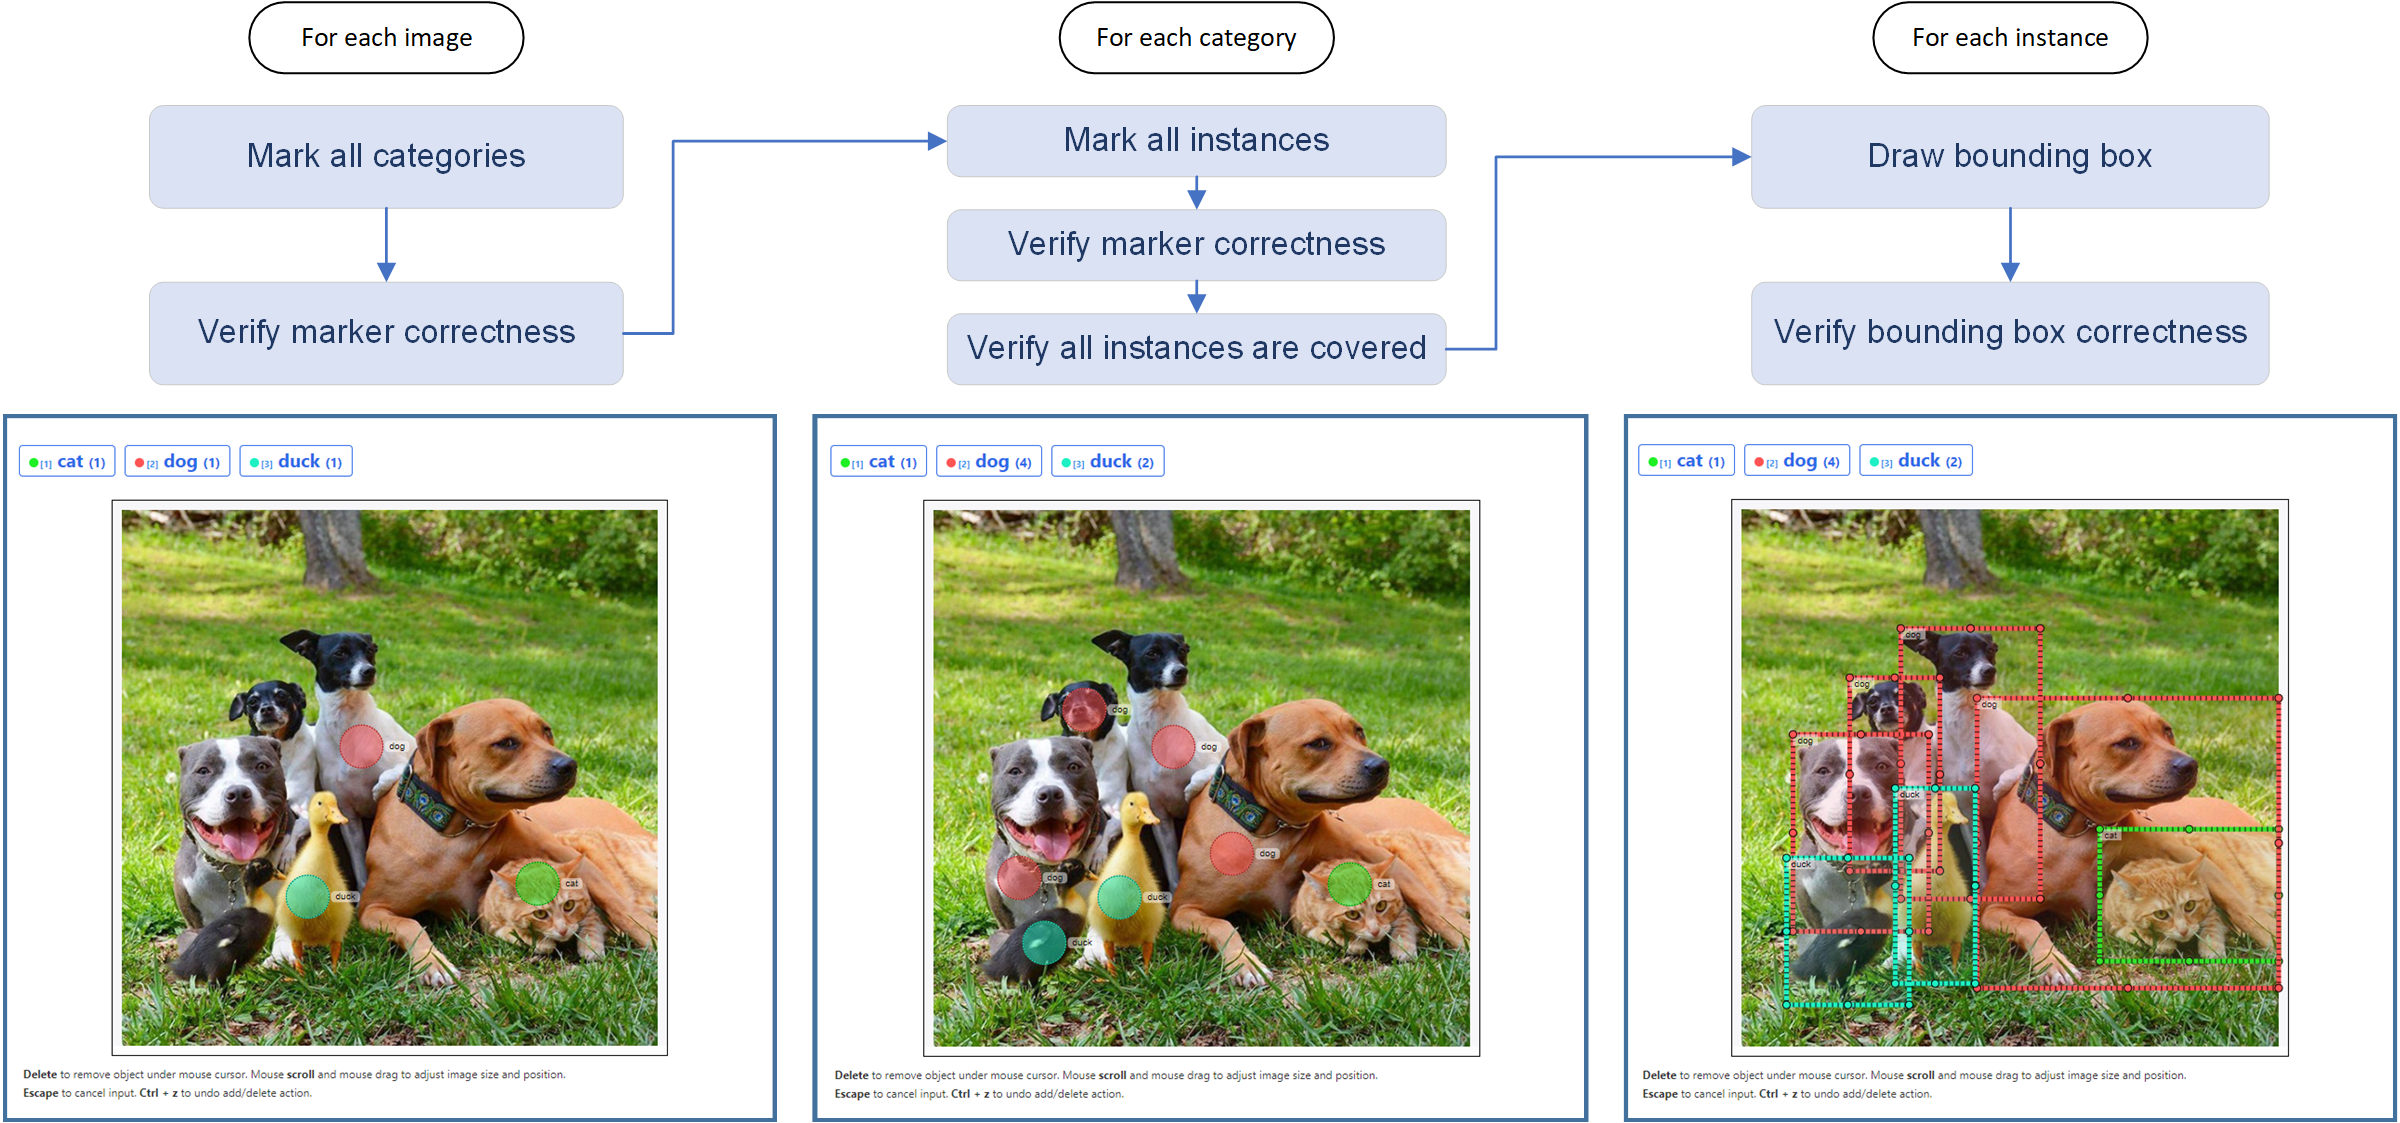
\includegraphics[width=0.9\linewidth]{images/bing_data_collection.png}
  \caption{\footnotesize{Data collection pipeline}}
  \label{fig:bing_data_collection}
\end{figure}

Рассмотрим подробнее шаги пайпплайна.

\paragraph{Category Discovery} В рамках первого шага задача состоит в том, чтобы просто определить какие категории объектов встречаются на изображении, без сообственно разметки объектов.
Для того чтобы упростить задачу, асессорам нужно определить \textit{одну новую категорию} на изображении, вместо того чтобы указывать сразу все категории (см. первую картинку на Рисунке~\ref{fig:bing_data_collection}).
Кроме того, чтобы выбор категории был максимально простым, в интерфейсе можно просматривать иерархию категорий.

После того как три асессора подряд не смогли выделить на изображении новую категорию считается, что определены все категории объектов на изображении. \\

Для того чтобы проверить качество выполнения данного шага, следом за category discovery следует \textit{verification micro-task} --- асессоров просят проверить правда ли что все выделенные категории действительно присутствуют на изображении.

\paragraph{Instance marking} Цель данного шага --- отметить объекты всех категорий, которые были выделены на прошлом шаге (см. вторую картинку на Рисунке~\ref{fig:bing_data_collection}). 

За данным шагом следует две \textit{verification micro-task}: 1) проверка того, что все объекты были отнесены к какой то категории 2) проверка того, что отмеченные объекты отнесены к верным категориям.

\paragraph{Bounding box drawing} Остается только нарисовать bounding box'ы вокруг отмеченных на прошлом шаге объектов (см. третью картинку на Рисунке~\ref{fig:bing_data_collection}).

Как и раньше, за данным шагом следует верификация --- асессоры проверяют, что bounding box'ы были нарисованы корректно. \\

Предложенный способ позволяет не только увеличить полноту (разметить большее число объектов), но так же позволяет это делать с меньшим бюджетом, в сравнении с задачей, когда асессоров сразу просят выполнить итоговую разметку объектов. \\

Кроме использования ручной разметки, авторы так же используют открытые датасеты.
Авторы объединяют все имеющиеся у них датасеты и выполняют \textit{class aware upsampling} для того чтобы сделать распределение категорий более равномерным. 
Это позволяет моделе научиться лучше распозновать редкие категории объектов, что очень важно для работы реальной системы.

\subsection*{Disjoint Detectors}

Для того чтобы можно было легко добавлять возможность распознования новых категорий объектов, не пребегая к необходимости полного переобучения модели, авторы предлгаюат обучать множество независимых детекторов для разных категорий объектов (\textit{disjoint detectors}), поверх общей модели (\textit{backbone}).

При таком подходе переобучать backbone модель нужно довольно редко, и можно очень просто добавлять модели для новых категорий или дообучать существующие детекторы. 
В результате, добавление новых детекторов не приводит к негативным изменениям в качестве распознования других категорий объектов.

\section*{Мое мнение}

Данная работа в лишний раз подтверждает тот факт, что для успеха ML решения очень важна качественная подготовка данных.
Кроме того, работа имеет, пожалуй, наиболее полное описание того как работают современные, масштабные VS системы.
Авторы описывают большое число челенджей и практические способы их решения.
Заинтерисованные читали найдут много интересного в оригинальной работе. \\

Пользуясь случаем, хочу порекомендовать курс от Яндекса, посвященный crowd платформам~\url{https://www.coursera.org/learn/practical-crowdsourcing}